\documentclass{beamer}\usepackage[]{graphicx}\usepackage[]{color}
%% maxwidth is the original width if it is less than linewidth
%% otherwise use linewidth (to make sure the graphics do not exceed the margin)
\makeatletter
\def\maxwidth{ %
  \ifdim\Gin@nat@width>\linewidth
    \linewidth
  \else
    \Gin@nat@width
  \fi
}
\makeatother

\definecolor{fgcolor}{rgb}{0.345, 0.345, 0.345}
\newcommand{\hlnum}[1]{\textcolor[rgb]{0.686,0.059,0.569}{#1}}%
\newcommand{\hlstr}[1]{\textcolor[rgb]{0.192,0.494,0.8}{#1}}%
\newcommand{\hlcom}[1]{\textcolor[rgb]{0.678,0.584,0.686}{\textit{#1}}}%
\newcommand{\hlopt}[1]{\textcolor[rgb]{0,0,0}{#1}}%
\newcommand{\hlstd}[1]{\textcolor[rgb]{0.345,0.345,0.345}{#1}}%
\newcommand{\hlkwa}[1]{\textcolor[rgb]{0.161,0.373,0.58}{\textbf{#1}}}%
\newcommand{\hlkwb}[1]{\textcolor[rgb]{0.69,0.353,0.396}{#1}}%
\newcommand{\hlkwc}[1]{\textcolor[rgb]{0.333,0.667,0.333}{#1}}%
\newcommand{\hlkwd}[1]{\textcolor[rgb]{0.737,0.353,0.396}{\textbf{#1}}}%
\let\hlipl\hlkwb

\usepackage{framed}
\makeatletter
\newenvironment{kframe}{%
 \def\at@end@of@kframe{}%
 \ifinner\ifhmode%
  \def\at@end@of@kframe{\end{minipage}}%
  \begin{minipage}{\columnwidth}%
 \fi\fi%
 \def\FrameCommand##1{\hskip\@totalleftmargin \hskip-\fboxsep
 \colorbox{shadecolor}{##1}\hskip-\fboxsep
     % There is no \\@totalrightmargin, so:
     \hskip-\linewidth \hskip-\@totalleftmargin \hskip\columnwidth}%
 \MakeFramed {\advance\hsize-\width
   \@totalleftmargin\z@ \linewidth\hsize
   \@setminipage}}%
 {\par\unskip\endMakeFramed%
 \at@end@of@kframe}
\makeatother

\definecolor{shadecolor}{rgb}{.97, .97, .97}
\definecolor{messagecolor}{rgb}{0, 0, 0}
\definecolor{warningcolor}{rgb}{1, 0, 1}
\definecolor{errorcolor}{rgb}{1, 0, 0}
\newenvironment{knitrout}{}{} % an empty environment to be redefined in TeX

\usepackage{alltt}

\mode<presentation>
{
 \usetheme{AnnArbor}
 \usecolortheme{crane}
}
\setbeamertemplate{navigation symbols}{}
\usepackage[english]{babel}
\usepackage{times}
\usepackage[T1]{fontenc}
\usepackage[applemac]{inputenc}
\usepackage{amsmath}


\setbeamerfont{caption}{size=\scriptsize}
\setbeamertemplate{caption}{\raggedright\insertcaption\par}
\usepackage{hyperref}  
\hypersetup{colorlinks=true,allcolors=blue}

\title[scRNA-seq de]{scRNA-seq}
\subtitle{Differential expression analysis methods}
\author[Olga]{Olga Dethlefsen}
\institute[NBIS]{NBIS, National Bioinformatics Infrastructure Sweden\\}
\date[October 2017]{October 2017}
\logo{
\includegraphics[height=0.8cm]{Images/nbislogo-orange.png}}
\IfFileExists{upquote.sty}{\usepackage{upquote}}{}
\begin{document}

\begin{frame}
\titlepage
\end{frame}

  % \item Introduction: where in scRNA-seq pipeline comes it handy to run DE, why this is not straighforward and why new approaches are needed and being developed
  % \item Common methods: what methods and papers are out there
  % \item Performance: how do we know which methods to choose (Dal Molin paper, statistical background, summary statsticis and simulated datasets, biological knowledge)
  % \item Summary and conclusions
  % \item Toy example 
  
  
\begin{frame}
\begin{block}{Outline}
\begin{itemize}
  \item Introduction: what is so special about DE with scRNA-seq
  \item Common methods: what is out there
  \item Performance: how to choose the best method
  \item Summary
  \item DE tutorial
 \end{itemize}
\end{block}
\end{frame}

\section{Introduction}

% Intro: Overview figure
\begin{frame}
\begin{center}
\begin{figure}
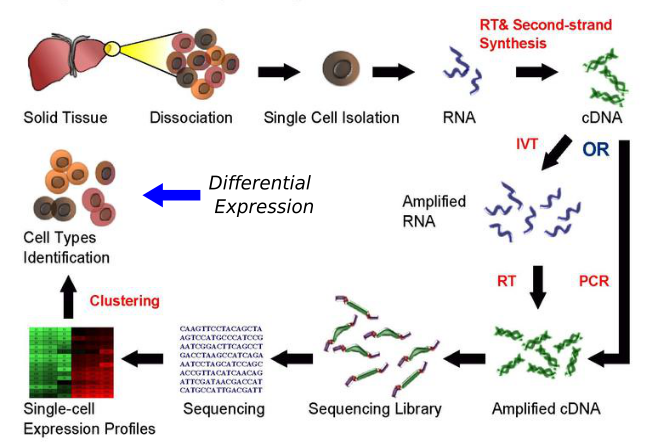
\includegraphics[width=10cm]{Images/DEoverview.png}
\caption{Figure: Simplified scRNA-seq workflow [adopted from \href{http://hemberg-lab.github.io/]}{http://hemberg-lab.github.io/}}
\end{figure}
\end{center}
\end{frame}


% Intro: Question
\begin{frame}
Differential expression is an old problem...so
\begin{block}{why is DE scRNA-seq different to RNA-seq?}
\begin{itemize}
  \item ?
  \item ?
  \item ?
  \item ?
  \item ?
 \end{itemize}
\end{block}
\end{frame}

% Intro: Reasons why scRNA-seq is different to bulk RNA-seq
\begin{frame}
Differential expression is an old problem...so
\begin{block}{why is DE scRNA-seq different to RNA-seq?}
\begin{itemize}
  \item scRNA-seq are affected by higher noise (technical and biological factors)
  \item low amount of available mRNAs results in amplification biases and "dropout events" (technical)
  \item 3' bias, partial coverage and uneven depth (technical)
  \item stochastic nature of transcription (biological)
  \item multimodality in gene expression; presence of multiple possible cell states within a cell population (biological)
 \end{itemize}
\end{block}
\end{frame}



\section{Common methods}

% Section slide
\begin{frame}
\begin{center}
\insertsection
\end{center}
\end{frame}


% CM: Triangle
\begin{frame}
\begin{center}
\begin{figure}
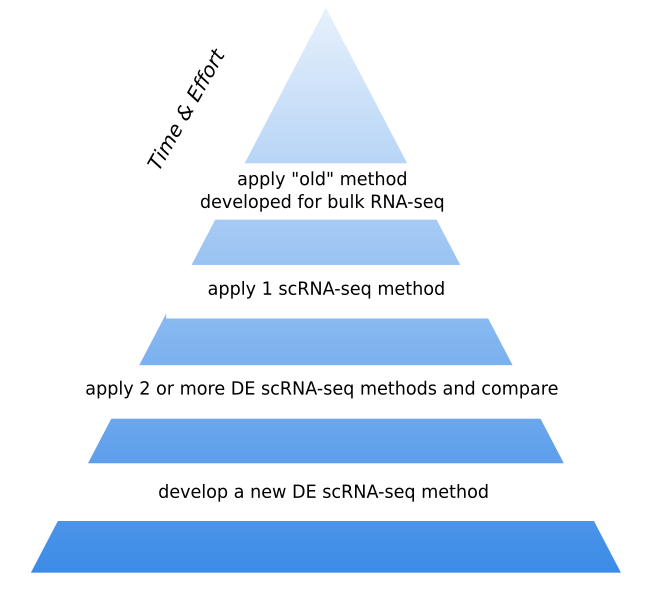
\includegraphics[width=10cm]{Images/solutionTriangle.png}
\caption{Simplified scRNA-seq workflow [adopted from \href{http://hemberg-lab.github.io/]}{http://hemberg-lab.github.io/}}
\end{figure}
\end{center}
\end{frame}

% CM: Name methods
\begin{frame}
\begin{block}{Common methods}
\begin{itemize}
  \item non-parametric test e.g. Kruskal-Wallis (generic)
  \item edgeR, limma (bulk RNA-seq)
  \item MAST, SCDE, Monocle (scRNA-seq)
  \item D$^3$E, Pagoda (scRNA-seq)
 \end{itemize}
\end{block}
\end{frame}

% CM: Miao Table 1
\begin{frame}
\begin{center}
\begin{figure}
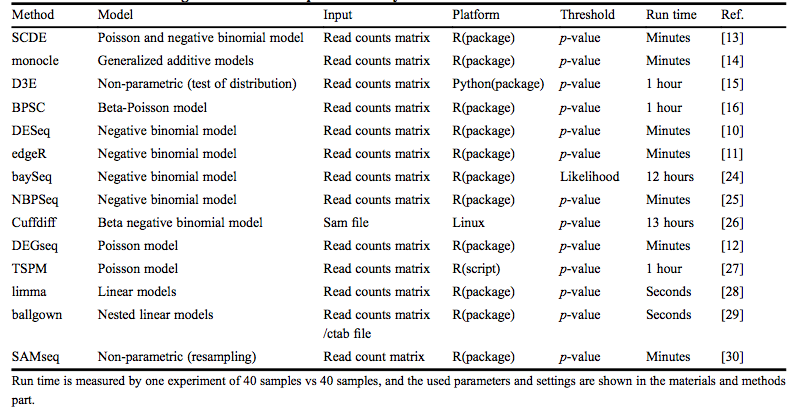
\includegraphics[width=10cm]{Images/MiaoTable1.png}
\caption{Table: Information of gene differential expression analysis methods used [Miao and Zhang, 2017, Quantitative Biology 2016, 4]}
\end{figure}
\end{center}
\end{frame}

% CM: Mast
\begin{frame}
\frametitle{MAST}
\begin{itemize}
  \item uses \href{https://onlinecourses.science.psu.edu/stat504/node/216}{generalized linear} \href{http://data.library.virginia.edu/getting-started-with-hurdle-models/}{hurdle model}
  \item designed to account for stochastic dropouts and bimodal expression distribution in which expression is either strongly non-zero or non-detectable
  \item The rate of expression \textbf{\textit{Z}}, and the level of expression \textbf{\textit{Y}}, are modeled for each gene \textbf{\textit{g}}, indicating whether gene \textbf{\textit{g}} is expressed in cell \textbf{\textit{i}} (i.e., $Z_{ig}=0$ if $y_{ig}=0$ and $z_{ig}=1$ if $y_{ig}>0$)
  \item A \href{https://stats.idre.ucla.edu/stata/webbooks/logistic/chapter1/logistic-regression-with-statachapter-1-introduction-to-logistic-regression-with-stata/}{logistic regression} model for the discrete variable \textbf{\textit{Z}} and a Gaussian linear model for the continuous variable (Y|Z=1):
   \end{itemize}
   \begin{center}
    $logit (P_r(Z_{ig}=1))=X_i\beta_g^D$ \newline
    $P_r(Y_{ig}=Y|Z_{ig}=1)=N(X_i\beta_g^C,\sigma_g^2)$, where $X_i$ is a design matrix
\end{center}
\begin{itemize}
\item Model parameters are fitted using an empirical Bayesian framework
\item Allows for a joint estimate of nuisance and treatment effects, DE is determined using the \href{https://onlinecourses.science.psu.edu/stat414/node/247}{likelihood ratio test}
\end{itemize}
\end{frame}


% CM: SCDE
\begin{frame}
\frametitle{SCDE}
\begin{itemize}
  \item models the read counts for each gene using a mixture of a NB, \href{https://onlinecourses.science.psu.edu/stat414/node/55}{negative binomial}, and a \href{https://onlinecourses.science.psu.edu/stat414/node/81}{Poisson} distribution 
  \item NB distribution models the transcripts that are amplified and detected
  \item Poisson distribution models the unobserved or background-level signal of transcripts that are not amplified (e.g. dropout events)
  \item subset of robust genes is used to fit, via \href{http://www.nature.com/nbt/journal/v26/n8/full/nbt1406.html?foxtrotcallback=true}{EM} algorithm, the parameters to the mixture of models
  \item For DE, the posterior probability that the gene shows a fold expression difference between two conditions is computed using a Bayesian approach
\end{itemize}
\end{frame}


% CM: Monocole
\begin{frame}
\frametitle{Monocole}
\begin{itemize}
\item Originally designed for ordering cells by progress through differentiation stages (pseudo-time)
\item The mean expression level of each gene is modeled with a \href{https://en.wikipedia.org/wiki/Generalized_additive_model}{GAM}, generalized additive model, which relates one or more predictor variables to a response variable as  
\end{itemize}
   \begin{center}
    $g(E(Y))=\beta_0+f_1(x_1)+f_2(x_2)+...+f_m(x_m)$ where Y is a specific gene expression level, $x_i$ are predictor variables, g is a link function, typically log function, and $f_i$ are non-parametric functions (e.g. cubic splines)
  \end{center}
\begin{itemize}  
\item The observable expression level Y is then modeled using GAM, 
\end{itemize}
$E(Y)=s(\varphi_t(b_x, s_i))+\epsilon$ where $\varphi_t(b_x, s_i)$ is the assigned pseudo-time of a cell and $s$ is a cubic smoothing function with three degrees of freedom. The error term $\epsilon$ is normally distributed with a mean of zero
\begin{itemize}
\item The DE test is performed using an approx. $\chi^2$ likelihood ratio test
\end{itemize}
\end{frame}


% CM: Let's stop for a minute
\begin{frame}
%\frametitle{SCDE}
Let's stop for a minute...
\begin{center}
\begin{figure}

\includegraphics[width=5cm]{Images/frustration.png}
%\caption{Simplified scRNA-seq workflow [adopted from \href{http://hemberg-lab.github.io/]}{http://hemberg-lab.github.io/}}
\end{figure}
\end{center}
\end{frame}

% CM: What is differential expression
\begin{frame}
\frametitle{Differential expression}
Differential expression analysis
\begin{itemize}
\item means taking the normalized read count data \&
\item performing statistical analysis to discover quantitative changes in expression levels between experimental groups. \item e.g. to decide whether, for a given gene, an observed difference in read counts is significant, that is, whether it is greater than what would be expected just due to natural random variation.
\item or simply: checking for differences in distributions
\end{itemize}
\end{frame}

% CM: The key: figure and equation
\begin{frame}
\frametitle{The key}
\begin{center}
\begin{figure}
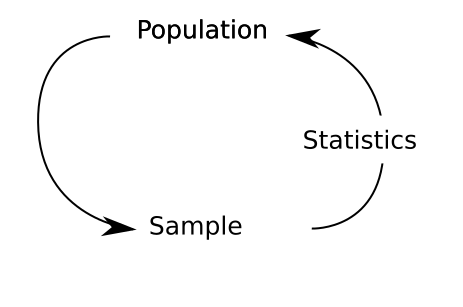
\includegraphics[width=5cm]{Images/stats.png}
\end{figure}
$Outcome_i=(Model_i)+error_i$
\end{center}
\begin{itemize}
\item we collect data on a \underline{\textit{sample}} from a much larger \underline{\textit{population}}. \underline{\textit{Statistics}} lets us to make inferences about the population from which it was derived
\item we try to predict the outcome given a model fitted to the data
\end{itemize}
\end{frame}

% CM: The key: t-test example
\begin{frame}
\frametitle{The key}
\begin{flushright}
$t=\frac{x_1-x_2}{s_p\sqrt{\frac{1}{n_1}+\frac{1}{n_2}}}$
\end{flushright}
\begin{knitrout}
\definecolor{shadecolor}{rgb}{0.969, 0.969, 0.969}\color{fgcolor}
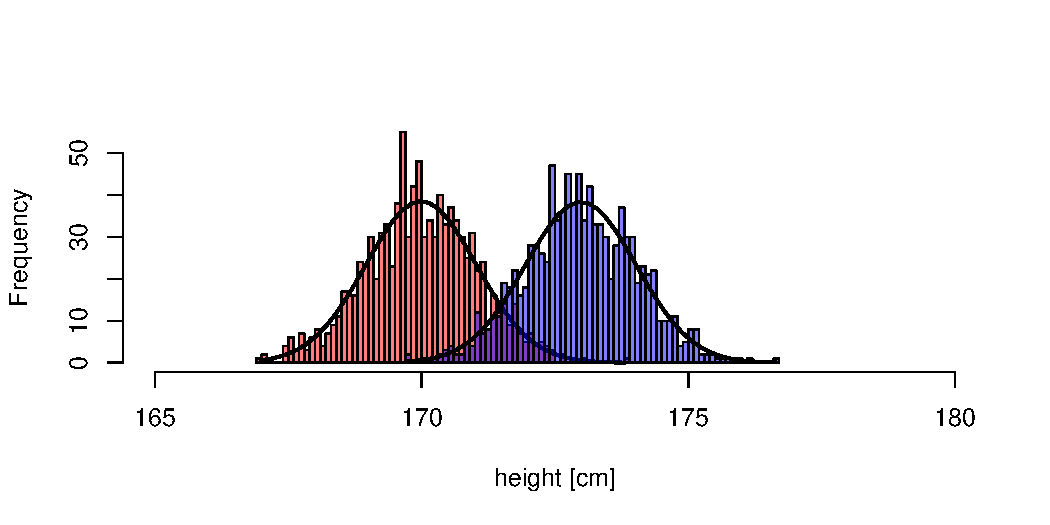
\includegraphics[width=\maxwidth]{figure/ttest-1} 

\end{knitrout}
\end{frame}


% CM: The most important equation
\begin{frame}
\frametitle{The key}
\begin{block}{Simple recipe}
\begin{itemize}
\item model e.g. gene expression with random error
\item fit model to the data and/or data to the model, estimate model parameters
\item use model for prediction and/or inference
\end{itemize}
\end{block}
% \begin{block}{Implications}
% \begin{itemize}
% \item the better model fits to the data the better statistics
% \end{itemize}
% \end{block}
\end{frame}

% CM: Mast 2
\begin{frame}
\frametitle{The key: MAST (again)}
\begin{itemize}
  \item uses \underline{generalized linear hurdle model}
  \item designed to account for stochastic dropouts and bimodal expression distribution in which expression is either strongly non-zero or non-detectable
  \item The rate of expression \textbf{\textit{Z}}, and the level of expression \textbf{\textit{Y}}, are modeled for each gene \textbf{\textit{g}}, indicating whether gene \textbf{\textit{g}} is expressed in cell \textbf{\textit{i}} (i.e., $Z_{ig}=0$ if $y_{ig}=0$ and $z_{ig}=1$ if $y_{ig}>0$)
  \item A \underline{logistic regression model} for the discrete variable \textbf{\textit{Z}} and a \underline{Gaussian linear model} for the continuous variable (Y|Z=1):
   \end{itemize}
   \begin{center}
    $logit (P_r(Z_{ig}=1))=X_i\beta_g^D$ \newline
    $P_r(Y_{ig}=Y|Z_{ig}=1)=N(X_i\beta_g^C,\sigma_g^2)$, where $X_i$ is a design matrix
\end{center}
\begin{itemize}
\item Model parameters are \underline{fitted} using an empirical Bayesian framework
\item Allows for a joint estimate of nuisance and treatment effects, \underline{DE is determined using the likelihood ratio test}
\end{itemize}
\end{frame}


% CM: SCDE 2
\begin{frame}
\frametitle{The key: SCDE (again)}
\begin{itemize}
  \item \underline{models} the read counts for each gene using a mixture of a NB, negative binomial, and a Poisson distribution 
  \item \underline{NB distribution} models the transcripts that are amplified and detected
  \item \underline{Poisson distribution} models the unobserved or background-level signal of transcripts that are not amplified (e.g. dropout events)
  \item subset of robust genes is used to fit, via \underline{EM} algorithm, the parameters to the mixture of models
  \item For DE, the posterior probability that the gene shows a fold expression difference between two conditions is computed using a \underline{Bayesian approach}
\end{itemize}
\end{frame}

% CM: Monocole 2
\begin{frame}
\frametitle{The key: Monocole (again)}
\begin{itemize}
\item Originally designed for ordering cells by progress through differentiation stages (pseudo-time)
\item The mean expression level of each gene is \underline{modeled with a GAM}, generalized additive model, which relates one or more predictor variables to a response variable as  
\end{itemize}
   \begin{center}
    $g(E(Y))=\beta_0+f_1(x_1)+f_2(x_2)+...+f_m(x_m)$ where Y is a specific gene expression level, $x_i$ are predictor variables, g is a link function, typically log function, and $f_i$ are non-parametric functions (e.g. cubic splines)
  \end{center}
\begin{itemize}  
\item The observable expression level Y is then modeled using GAM, 
\end{itemize}
$E(Y)=s(\varphi_t(b_x, s_i))+\epsilon$ where $\varphi_t(b_x, s_i)$ is the assigned pseudo-time of a cell and $s$ is a cubic smoothing function with three degrees of freedom. The error term $\epsilon$ is normally distributed with a mean of zero
\begin{itemize}
\item The DE test is performed using an \underline{approx. $\chi^2$ likelihood ratio test}
\end{itemize}
\end{frame}

% CM: The key implications
\begin{frame}
\frametitle{They key: implication}
\begin{block}{Simple recipe}
\begin{itemize}
\item model e.g. gene expression with random error
\item fit model to the data and/or data to the model, estimate model parameters
\item use model for prediction and/or inference
\end{itemize}
\end{block}
\begin{block}{Implication}
\begin{itemize}
\item the better model \href{http://www.itl.nist.gov/div898/handbook/pmd/section4/pmd44.htm}{fits} to the data the better statistics
\end{itemize}
\end{block}
\end{frame}

% CM: Distributions
\begin{frame}
\begin{knitrout}
\definecolor{shadecolor}{rgb}{0.969, 0.969, 0.969}\color{fgcolor}
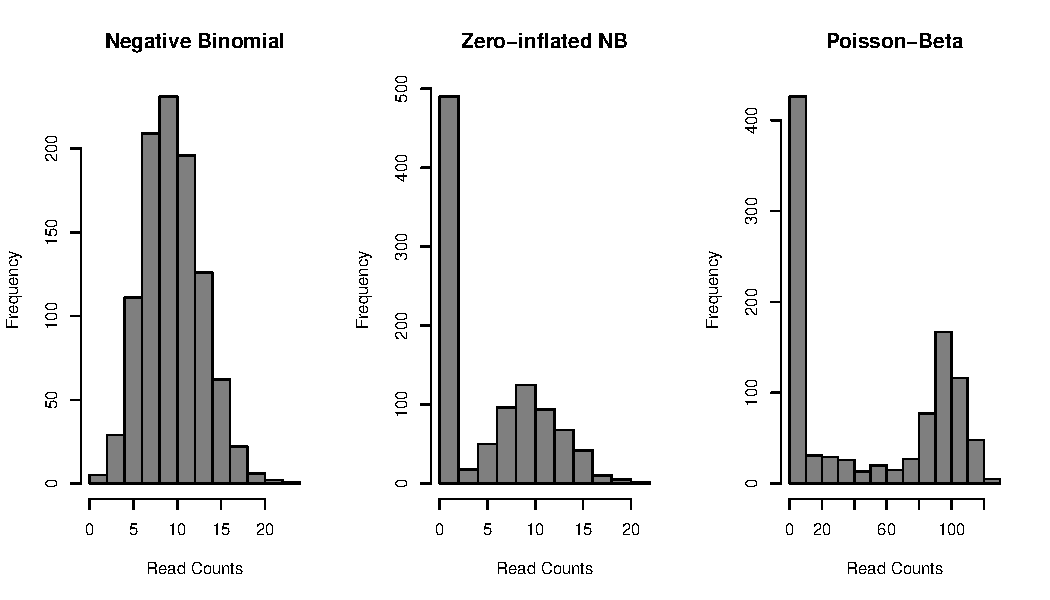
\includegraphics[width=\maxwidth]{figure/dist-1} 

\end{knitrout}
\end{frame}

\section{Performance}
\begin{frame}
\begin{center}
\insertsection
\end{center}
\end{frame}

% P: no golden standard
\begin{frame}
\frametitle{No golden standard}
There is no golden standard, no single best solution
\newline
\newline
...so what do we do?
\newline
\newline
\begin{flushright}
\pause we gather as much evidence as possible
\end{flushright}
\end{frame}

% P: assess data and distributions
\begin{frame}
\frametitle{Get to know your data \& wisely choose DE methods}
Example data: 46,078 genes x 96 cells \newline
22,229 genes with no expression at all

\begin{knitrout}
\definecolor{shadecolor}{rgb}{0.969, 0.969, 0.969}\color{fgcolor}
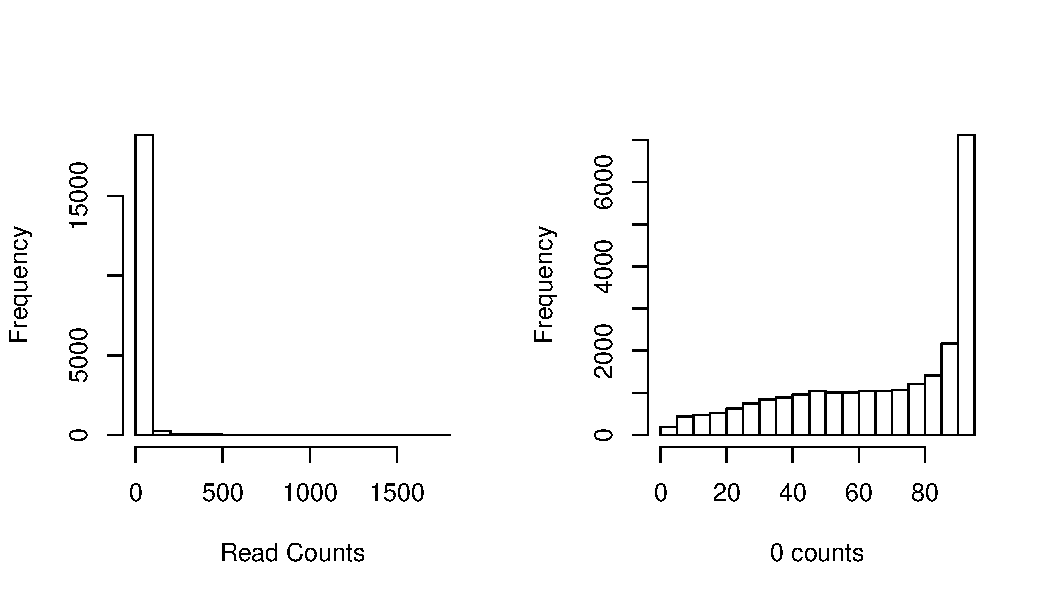
\includegraphics[width=\maxwidth]{figure/knowdata-1} 

\end{knitrout}
\end{frame}

% P: Dal Molin
\begin{frame}
\frametitle{Learn from methodological papers and/or past studies}
e.g. \href{https://www.frontiersin.org/articles/10.3389/fgene.2017.00062/full(}{Dal Molin, Barruzo and Di Camilillo, frontiers in Genetics 2017, Single-Cell RNA-Sequencing: Assessment of Differential Expression Analysis Methods}
\begin{itemize}
\item 10,000 genes simulated for 2 conditions with sample size of 100 cells each
\item 8,000 genes were simulated as not differentially expressed using the same distribution (unimodal: NB and bimodal: two-component NB mixture)
\item 2,000 genes were simulated as differentially expressed according to four types of differential expressions 
\item real dataset: 44 mouse Embryonic Stem Cells and 44 Embryonic Fibroblsts for positive control
\item real dataset: 80 single cells as negative control
\end{itemize}
\end{frame}

% P: Dal Molin plots
\begin{frame}
\frametitle{Learn from methodological papers and/or past studies}
\begin{center}
\begin{figure}
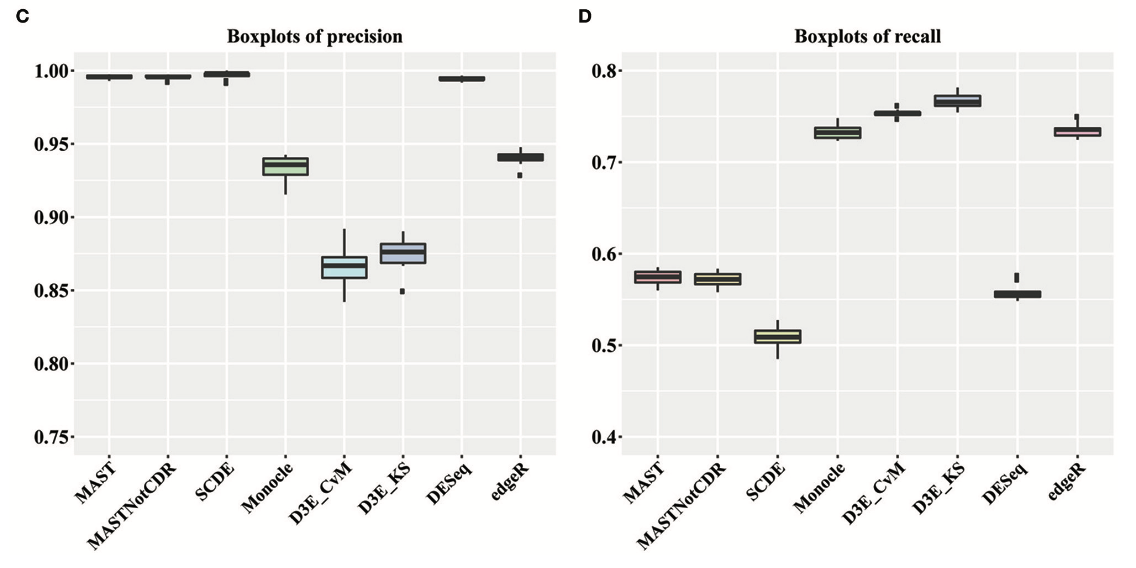
\includegraphics[width=12cm]{Images/DalMolin_fig2cd.png}
\end{figure}
\end{center}
\end{frame}

% P: Miao
\begin{frame}
\frametitle{Compare methods}
e.g. \href{Differential expression analyses for single-cell RNA-Seq: old questions on n???}{Miao and Zhang, Quantitative Biology 2016,4: Differential expression analyses for single-cell RNA-Seq: old questions on new data}
\begin{center}
\begin{figure}
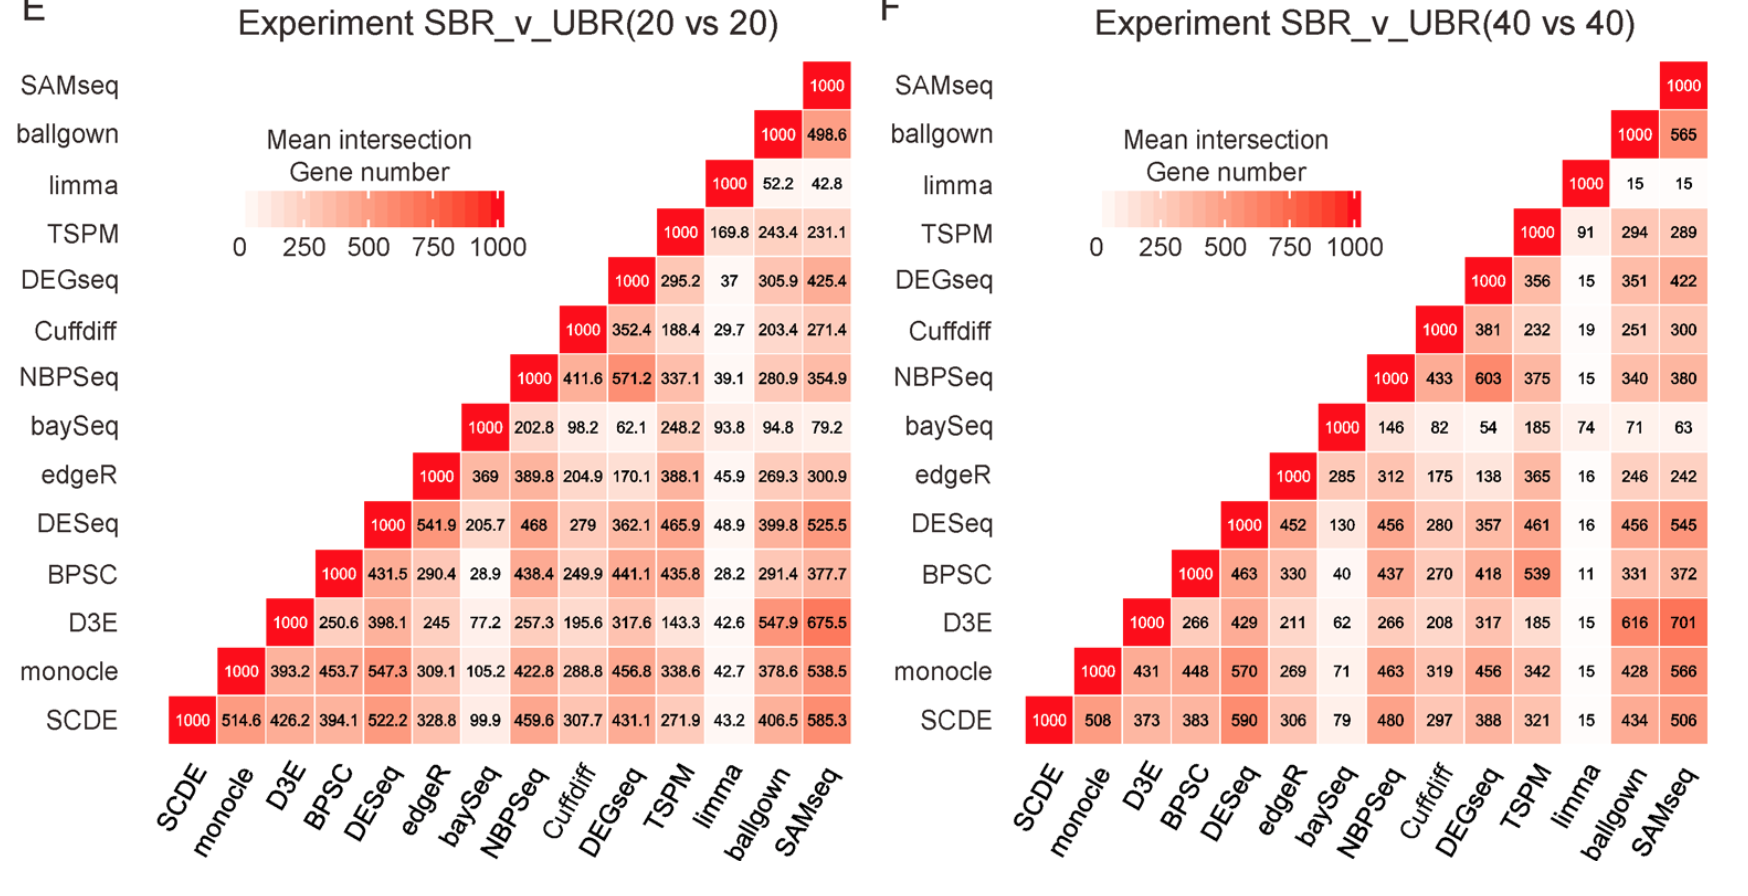
\includegraphics[width=11cm]{Images/Miao_fig1ef.png}
\end{figure}
\end{center}
\end{frame}

% P: Stay critical
\begin{frame}
\frametitle{Stay critical}
\begin{center}
\begin{figure}
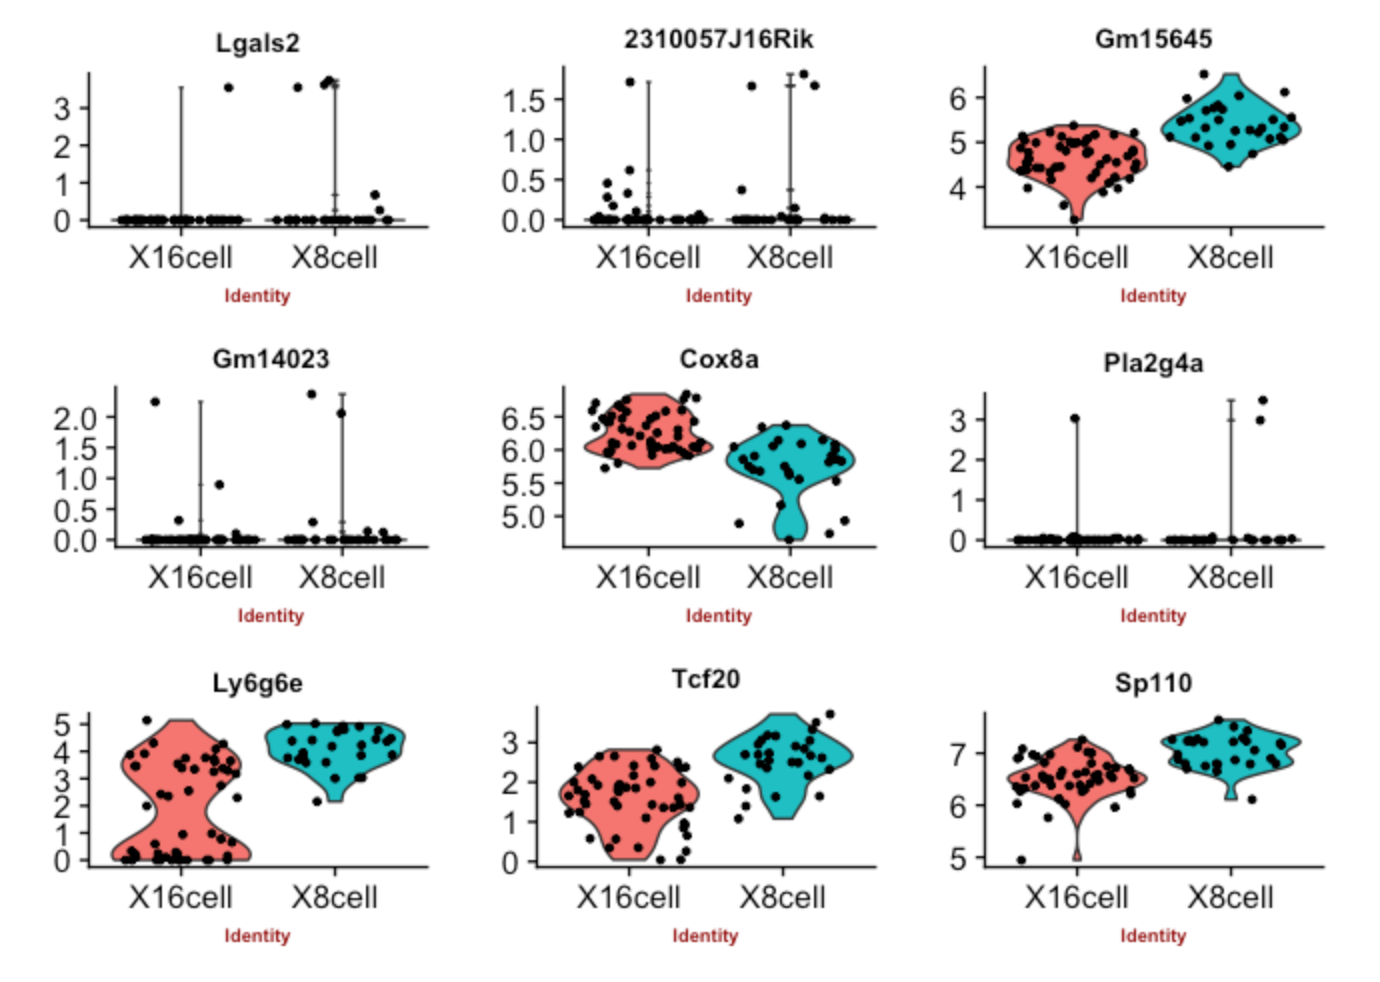
\includegraphics[width=11cm]{Images/asa1.png}
\end{figure}
\end{center}
\end{frame}

% Summary section
\section{Summary}
\begin{frame}
\begin{center}
\insertsection
\end{center}
\end{frame}

% Summary points
\begin{frame}
\begin{block}{Summary}
\begin{itemize}
\item scRNA-seq is a rapidly growing field
\item DE is a common task so many newer and better methods will be developed
\item think like a statistician: get to know your data, think about distributions and models best for your data. Avoid applying methods blindly
\item comparing methods is good as long as you are aware what you are comparing and why
\item stay critical
\end{itemize}
\end{block}
\end{frame}

% Tutorial
\section{DE tutorial}
\begin{frame}
\begin{center}
\insertsection
\end{center}
\end{frame}

% Tutorial points
\begin{frame}
\begin{block}{DE tutorial}
Based on the dataset used is single-cell RNA-seq data (SmartSeq) from mouse embryonic development from Deng. et al. Science 2014, Vol. 343 no. 6167 pp. 193-196, "Single-Cell RNA-Seq Reveals Dynamic, Random Monoallelic Gene Expression in Mammalian Cells".
\begin{itemize}
\item check for differentially expressed genes between 8-cell and 16-cell stage embryos
\item with many methods incl. SCDE, MAST, SC3 package, Pagoda, Seurat
\item and compare the results, trying to decide on the best DE method for the dataset
\end{itemize}
\end{block}
\end{frame}

\section{Finally}
\begin{frame}
\begin{center}
Thank you for attention
\newline
\newline
Questions?
\newline
\newline
Enjoy the rest of the course
\newline
\newline
olga.dethlefsen@nbis.se
\end{center}
\end{frame}


\end{document}
